\documentclass[12pt]{article}
\usepackage{../template/NotesTeX}
\usepackage{physics}
\graphicspath{ {/home/ab/school/notes/chemmat121/} }
\begin{document}

\title{Chemmat 121}
\author{Alexander Bailey}
\emailAdd{alexkingstonbailey@gmail.com}
\maketitle
\flushbottom

\section{Deformation and structure of solids}
\subsection{Strength}
How much force can a material withstand before it fails?
That's a materials strength.
A material can fail in several ways but the two most common are fracturing and permanent deformation.

  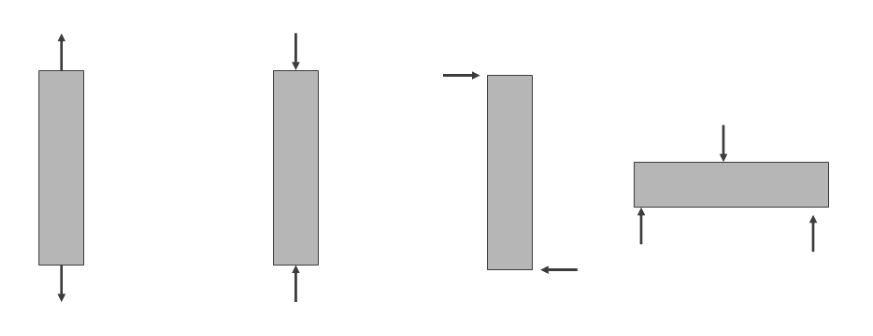
\includegraphics[scale=0.5]{force-types}
  \begin{center}
    Some types of force that a material/object can undergo

    From left: Tension, Compression, Shear and a Combination.
  \end{center}

\subsection{Stress}
Engineers typically talk about stress instead of forces because stress is just a force proportional to its area.
Stress is represented by the greek letter sigma ($\sigma$) and is given by the force (F) divided by the cross-sectional area (A).

\marginnote{Cross-sectional area is the area that is perpendicular to the applied force}

\begin{equation*}
  \sigma = \frac{F}{A} \\
\end{equation*}

\begin{example}
  \begin{flalign*}
    \text{Given: } m=25\unit{kg}, d=10\unit{mm} \\
    A = \pi r^2 \\
    A = \pi \times \frac{(0.01)^2}{2} \\
    F = 25 \times 9.81 \\
    \sigma = \frac{F}{A} \\
    \sigma = 3,120,000 \unit{Pa} \\
    \sigma = 3.12 \unit{MPa} \\
  \end{flalign*}
\end{example}

\begin{marginfigure}
  \vspace{-8cm}
  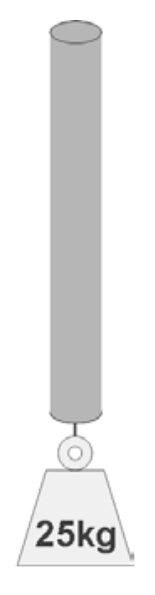
\includegraphics[scale=0.3]{stressexample}
\end{marginfigure}

\subsection{Strain}
Strain is how long something gets compared to its original size.
Stress and strain are related very closely and the stress against strain graph is a very important thing to materials engineering.
Strain is given by the change in length over the original length.

\begin{equation*}
  \epsilon = \frac{\Delta L}{L_o} 
\end{equation*}  

Strain is unitless but is commonly expressed as a percentage (\%).

\begin{example}
  \begin{align*}
    \epsilon &= \frac{\Delta L}{L_o} \\
             &= \frac{100.32\unit{mm}-100\unit{mm}}{100\unit{mm}} \\ 
            &= \frac{0.32\unit{mm}}{100\unit{mm}} \\ 
            &= 0.0032 \\
            &= 0.32\% \\ 
  \end{align*}
\end{example}

\subsection{Stress-Strain Curve}
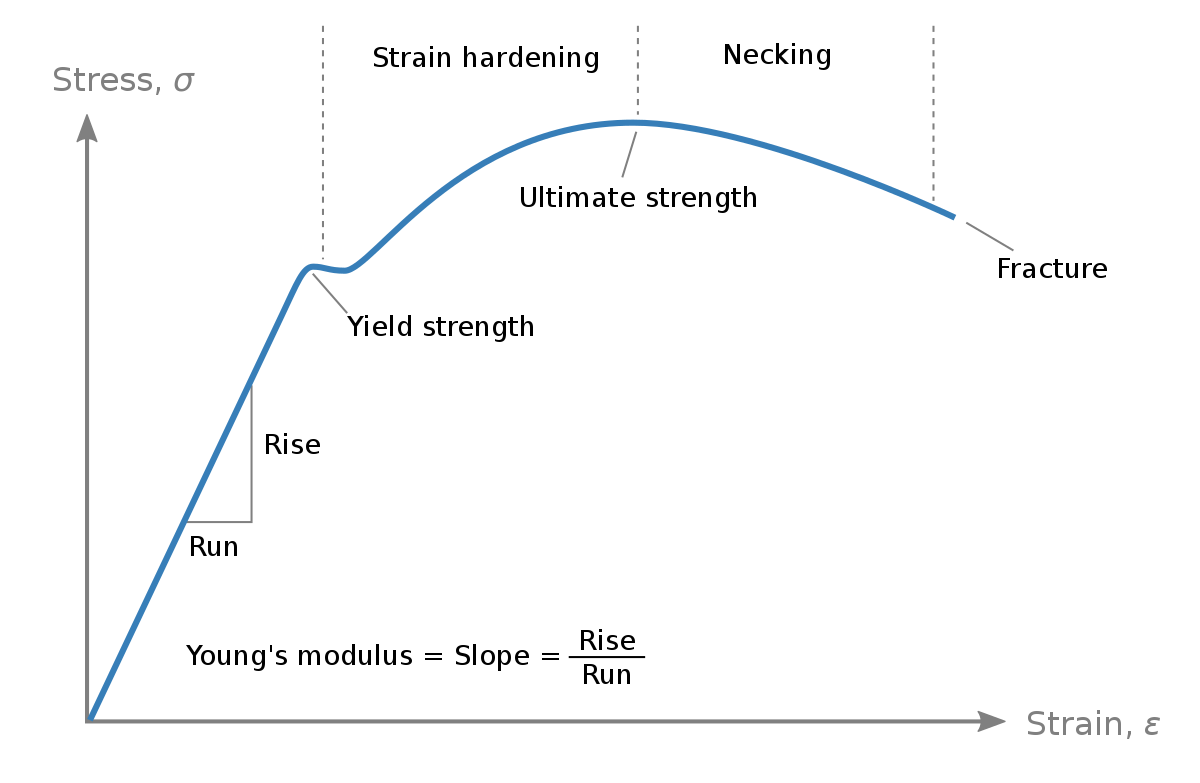
\includegraphics[scale=0.3]{stressvsstrain}

\en{The area under the curve is $F\times d$ and gives the `toughness' which is approximately the energy required.}[-8cm]

\en{Necking is a localised reduction in thickness, which reduces diameter, which reduces area, increasing stress. This causes it to fail.}[-4cm]

\subsection{Poisson's Ratio}
Poisson's ratio is the relationship between deformation for a given material. 
It is a measure of the Poisson effect, that describes the expansion or contraction of a material in directions perpendicular to the direction of loading. 
It has no units and is represented by the greek character `nu' ($\nu$).
For most materials $\nu \approx 0.3$.

\begin{equation*}
\nu = \frac{-\epsilon_x}{\epsilon_z}
\end{equation*}

\subsection{Young's Modulus}
The Young's Modulus of a material is a measure of the `stiffness'. 
It is the gradient of the elastic part of the stress-strain curve for a given material.
It has units of Pascals (Pa) and is represented by the capital letter E. 

\begin{equation*}
  E = \frac{\Delta \sigma}{\Delta \epsilon} 
\end{equation*}
\subsection{Steel}
Steel has what is called a `discontinuous yield'.  
This means at the yield strength there is a bit of `noise' and it moves a little randomly before becoming nonlinear. 

\subsection{0.2\% Proof Stress}
The 0.2\% Proof Stress of a material is a geometrical construct that is used when the yield stress of a material cannot be properly determined. 
It is a very slight overestimate (generally) that can be calculated by drawing a line parallel to the actual curve at a strain of $0.002$ and finding the intersection with the original curve.
This stress value is the approximation. 

\subsection{Safety Factor}
The safety factor is a scalar value that demonstrates how much more stress a material can hold relative to the requirement. 
I.e. if, for example, $F \approx 1000\unit{N}$ the engineers might pretend $F = 2000N$. 
This would gie a safety factor of 2.

When the conditions of the material are more uncertain, you would want a higher safety factor.

\subsection{Engineering Stress vs Real Stress}
In engineering, we draw a stress-strain graph as going `down' after the ultimate tensile strength.
In reality, because of the effect of necking, it goes up after this.
As engineers, we use the model because it is easier to handle theoretically.

\subsection{Ductility}
Ductility is a measure of how much something can deform elastically (with 100\% recovery / without permanent deformation).
The stress-strain graph of a ductile material will have a longer elastic section while a more brittle material (less ductile) will have a shorter one.
It is generally described by one of two equations: 

\begin{center}
  \textbf{Percentage Elongation}
\end{center}
\begin{equation*}
  = \frac{\Delta L}{L_o} \times 100\% 
\end{equation*}

\begin{center}
  \textbf{Percentage Reduction in Area}
\end{center}
\begin{equation*}
  = \frac{\Delta A}{A_o} \times 100\% 
\end{equation*}

\section{Microstructure and mechanical properties}
\subsection{Crystal Structure}
\begin{definition*}
  If a material is crystalline, the atoms of a material have \textbf{LONG RANGE ORDER}. 
  This means the material is made up of a crystal lattice made of repeating units called `unit cells'. 
\end{definition*}

There are 14 possible crystal arrangements but this course will only look at three. 
We describe arrangements by looking at the unit cell. 
The unit cell is a tessellating shape that has all the information to describe the entire lattice.

The unit cell has 4 important properties: 
\begin{itemize}
  \item Number of atoms 
  \item Co-ordination Number (The number of neighbours for the unit cell)
  \item Unit Cell Dimension (The length of each side of the cell written `a')
  \item Atomic Packing Factor (Amount of space taken up by the atoms)
\end{itemize}

\begin{equation*}
  a = \text{ Atomic Packing Factor } = \frac{\text{volume of atoms}}{\text{volume of unit cell}}
\end{equation*}

\subsubsection{Body Centered Cubic} 
Body Centered Cubic (BCC) has one atom at each corner of a cube and one right in the middle.
\begin{marginfigure}
  \vspace{ -1cm }
  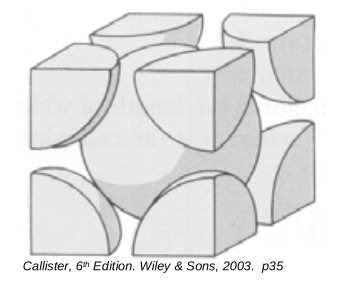
\includegraphics[scale=0.15]{bcc}
\end{marginfigure}

\begin{itemize}
  \item Number of Atoms = $2 = 1 + 8 \times \frac{1}{8}$
  \item Co-ordination Number = 8 
  \item Unit cell dimension = $\frac{4R}{\sqrt{3}}$
  \item APF = 0.68 = 0.68\%
\end{itemize}

\subsubsection{Face Centered Cubic}
Face Centered Cubic (FCC) has one atom at each corner of a cube and one in the middle of each face of the cube.
\begin{marginfigure}
  \vspace{ -1cm }
  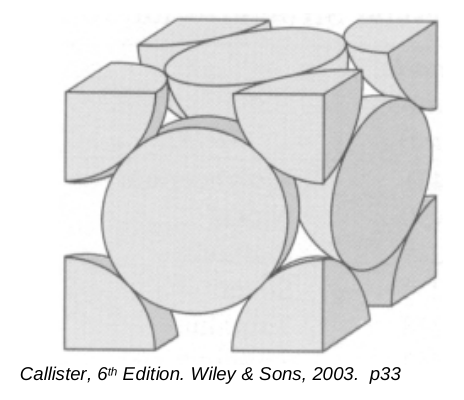
\includegraphics[scale=0.11]{fcc}
\end{marginfigure}

\begin{itemize}
  \item Number of Atoms = $4$
  \item Co-ordination Number = 12 
  \item unit cell dimension = $\frac{4R}{\sqrt{2}}$
  \item APF = 0.74 = 0.74\%
\end{itemize}

\subsubsection{Hexagonal Close Packed}
Hexagonal Close Packed (HCP) is a prism shape with hexagonal arrangements of atoms layered up.
\begin{marginfigure}
  \vspace{ -1cm }
  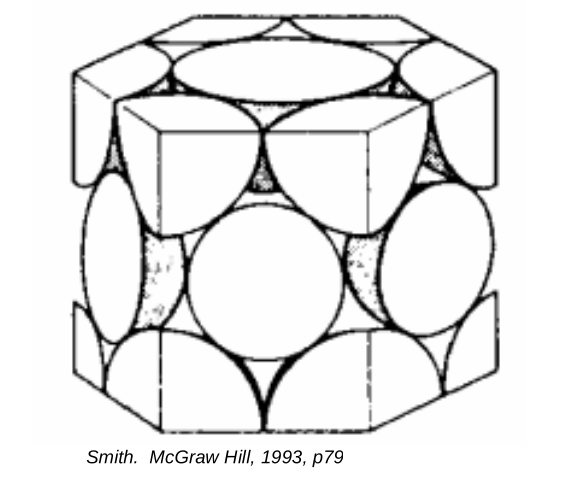
\includegraphics[scale=0.1]{hcp}
\end{marginfigure}

\begin{itemize}
  \item Number of Atoms = $6$
  \item Co-ordination Number = 12 
  \item APF = 0.74 = 0.74\%
\end{itemize}

\subsection{Density}
Density is the degree of compactness of a substance. 
The amount of mass you get for a given volume.
The density of a material is its mass divided by its volume.
\begin{equation*}
  \rho = \frac{n.A}{V_c.N_a}
\end{equation*}
Where $n$ is the number of atoms per unit cell, $A$ is the atomic mass of the material, $V_c$ is the volume of the unit cell ($a^3$) and $N_a$ is Avrogado's Number.

\begin{example}
  Iron
  \begin{gather*}
    a = 0.286\unit{nm }, n = 2 \\
    \rho = \frac{ 2 \times 55.85 }{(2.86\times10^{-8})^3 \times 6.023 \times 10^{23}} \\
    \rho = 7.92\unit{g.cm}^{-3}
  \end{gather*}
  The real density of iron is 7.87$\unit{g.cm}^{-3}$ so this is a good estimate.
\end{example}

\subsection{Polymorphism}
Materials that can exist in more than one crystal form (can have lattices made up of different unit cells) are called polymorphic. 
For example, Iron at room temperature has a BCC structure but at $912^\circ$C it has an FCC structure.

\newpage
\subsection{Planes, Directions and Positions}
Navigation around our crystal structures is based on a typical x,y,z orthogonal axis. 
We can denote the postition of an atom using a typical three dimensional vector. 
By convention, positions are denoted with round brackets.

\begin{marginfigure}
  \vspace{-1.5cm}
  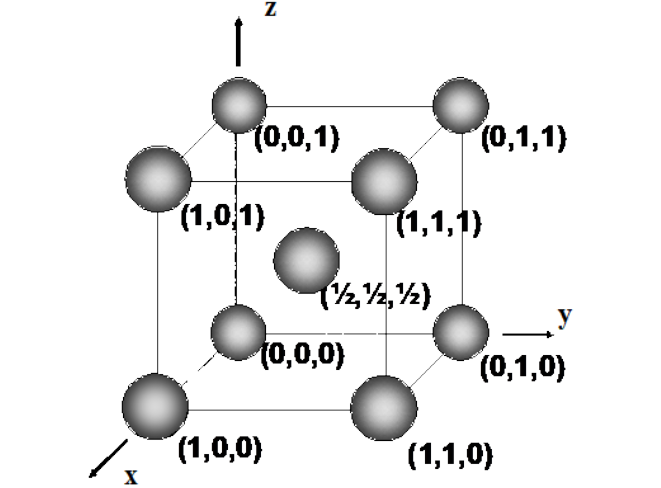
\includegraphics[scale=0.2]{positions}
\end{marginfigure}


\subsubsection{Directions}
Directions in the lattice are defined with square brackets $[u,v,w]$.

\begin{enumerate}
  \item Draw a vector from the origin for the direction 
  \item Project the length of the vector onto the unit cell axes 
  \item Put this in terms of the coefficients 
  \item Convert to integers (multiply by a constant)
  \item Put in square brackets 
\end{enumerate}

\begin{example}
  Projecting the length of the vector onto axes:
  $1a$ $0b$ $\half c$

  Put this in terms of co-efficients:
  $1$ $0$ $\half$

  Convert to integers (multiply by two):
  2 0 1

  Put in square brackets:
  $[201]$
\end{example}

Note: Negative directions will have a bar over them (read `bar').  

\begin{equation*}
[1\bar{1}0]
\end{equation*}

\subsubsection{Planes}
Planes in the lattice are defined by \textbf{Miller Indices} $(h,k,l)$.

\begin{enumerate}
  \item Ensure the origin is not on the plane 
  \item Determine distance to to intercept plane, by travelling along each axis from the origin (intercepts)
  \item Take reciprocals of the intercepts 
  \item Convert to integers (multiply by a constant)
  \item Put in round brackets (parenthesis)
\end{enumerate}

\begin{example}
  Intercepts: $1$ $-1$ $\infty$

  Reciprocals: $1$ $-1$ $0$

  Integers: $1$ $-1$ $0$

  Round Brackets: $(1\bar{1}0)$
\end{example}

\subsubsection{Families}
You can denote the `family' of a plane (all of the planes made up with these values). 
Families of planes are denoted with curly brackets e.g. Cube Faces $\{100\}$.
Families of directions are denoted with angle brackets e.g. $<100>$.

\subsection{Slip, Theoretical Strength and Defects}
Recall that there are two types of deformation: Elastic and Plastic (In-elastic).
Elastic Deformation springs back (recovers), Plastic Deformation does not.

At the atomic level, Elastic Deformation is merely stretching the atomic bonds.
Any further deformation is permanent (plastic, past the yield point) and results from a process called \textbf{slip}.
In plastic deformation, atomic bonds are broken (and remade).

\subsubsection{Theoretical Strength}
We can can calculate the \textit{theoretical} strength of a material by evaluating the amount of energy needed to break and remake the atomic bonds.
This is not a very good approximation. For example, the theoretical shear strength of pure iron is 10,000MPa but the measured shear strength of pure iron is 20MPa...
Why is this? Imperfections.

\subsection{Imperfections}
There are a number of a different imperfections that DO happen within a lattice containing millions of atoms.
This is what causes our theoretical strength and theoretical density to be off. 
It is EXTREMELY difficult to get `pure' anything so this is true for any sample.

\begin{itemize}
  \item Point Defects
    \begin{itemize}
      \item Vacancy
      \item Substitution
      \item Interstitial Atom
    \end{itemize}
  \item Planar Defects (Dislocations, $\bot$)
    \begin{itemize}
      \item Edge Dislocation
      \item Screw Dislocation
    \end{itemize}
\end{itemize}

A vacancy is simply a missing atom in the lattice.
A substitution is when a different atom is in the place of the atom that should be there. 
Interstitial atoms are atoms that occupy a normally unoccupied site in a crystal lattice.

\subsection{Slip}
\begin{center}
  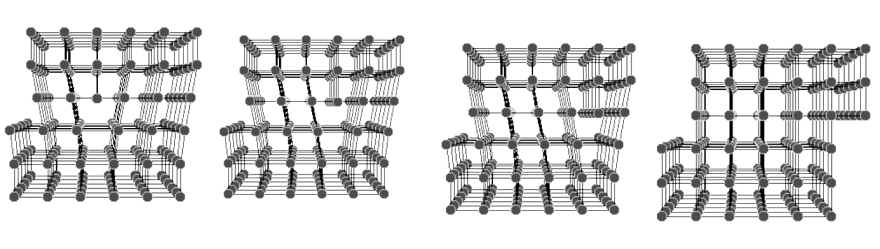
\includegraphics[scale=0.2]{slip}
\end{center}

\marginnote{Explaining how Slip works is a common exam question. Draw these!}[-1.7cm]

The model of slip we will use is the movement of dislocations.
The movement of dislocations means that slip can occur more easily than in a perfect arrangement of atoms.
Easy slip means that a material is easily plastic deformed, this means it is \textit{ductile}.


\subsubsection{Slip Systems}
Slip (dislocation movement) occurs most easily on closepack planes and in closepacked directions.
Not all systems have closepacked planes so slip happens on the \textit{closest} packed plane  

A slip system is a combination of planes and directions.
For FCC, the closepacked planes are $\{111\}$\mn{A family of planes}.
The closepacked directions on these planes are $<110>$\mn{A family of directions}.

Hence, the main slip system for FCC is: $\{111\}<110>$

The main slip system for BCC is: $\{110\}<111>$

HCP structures have closepacked planes but they are all parallel.
Slip is very difficult so HCP metals are often brittle. 

\subsection{Microstructure}
Engineering components are very rarely single crystals, this means they are polycrystalline (many crystals).
Most metals have at some point been molten and as they solidify they form many crystals.

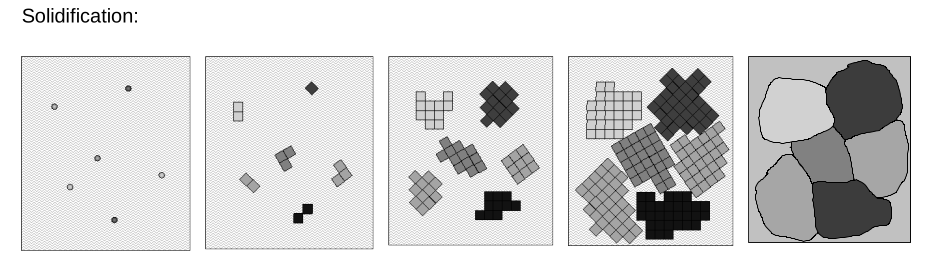
\includegraphics[scale=0.4]{solidification}

The name for the individual pieces is nucleus.
If they have lost enough energy (cooling down) they might form nuclei when they bump together.
This happens in the 2nd panel, you can call them "Baby Crystals".

The separate sections are `perfect crystals' (but they still contain defects) and in the 4th panel they are \textbf{equiaxed}. 
This means they are roughly equal in each axis and of the same size (roughly spherical/of the same size).
Each one of these crystals is called a `grain'.  
We can then talk about \textbf{Grain Structures} within a metal and \textbf{Grain Boundaries}.

When one grain meets another, the atoms are not perfectly aligned. 
This means there is a little extra energy due to the atomic bonds being incomplete or out-of-equilibrium.
This makes the grain boundary a `high energy region'.

\subsubsection{Nucleation}
When the grains form from a molten state it is called \textbf{nucleation}. 
This can occur on another solid material or in solution. 
It is quite rare to occur in solution on its own but it is called \textbf{Homogeneous Nucleation}.
When it forms on a surface e.g. the side of a mould it is called \textbf{Heterogeneous Nucleation}.

\subsection{Casting}
\subsubsection{Sand Casting}
Sand Casting is an ancient method of casting. 
You use something (foam etc) to make a hole in the sand and then fill your `runner' (input) with molten metal until it burns away all the filler.
This will then set in the sand you can take off the `cope' or `drag' (bottom or top) and access your new sword or cannon or frypan!

\begin{center}
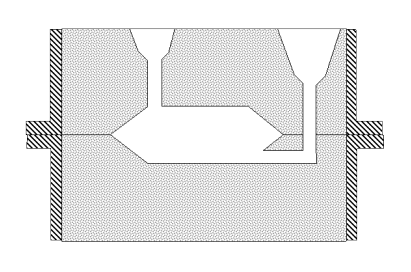
\includegraphics[scale=0.8]{sandcasting}
\end{center}
\subsubsection{Die Casting}
Die casting is a much more expensive modern method of casting.
In die casting, a permanent mould is created using machining tools out of another metal.
These moulds can be hundreds of thousands of dollars.
All forms of casting are prone to porosity however, weakening the part.

\subsection{Grain Structure Development}
Grains will mostly nucleate on the sides (walls) of the mould.
The first grains you will get are equiaxed grains.
Columnar grains will form in `columns' and stretch across the mould, possible touching the grains on the other side.
Sometimes columnar grains will form branches, these are called dendrite formations.
\marginnote{Frost will also form dendrites when it goes from gas to solid.}[-1cm]

\subsection{Metallography} 
Metallography is the study of the structure of metals. 
We use a reflective-light microscope (instead of a transmission microscope) because the metal is far too opaque to use a transmission scope.
Before we can use a microscope however you must prepare the surface.
This is to make the rough, cut surface smooth and reflective.

To allow us to see the grain boundaries, we `etch' the metal with an acid or alkali that selectively `attacks' the boundaries.
This means the boundaries will scatter light instead of reflecting it so they appear dark under the microscope. 
\marginnote{Some of the grains appear darker because they are also attacked by etching}
The general preparation process is

\begin{enumerate}
  \item Grinding
  \item Polishing (using finer and finer abrasives)
  \item Etching
  \item Cleaning (with hair-dryer, water, etc)
\end{enumerate}

\subsection{Grain Boundaries and dislocation movement}
More grains strengthen the metal because the grain boundaries stop dislocation movement (slip).
There is hence a relationship between the grain diameter and yield stress. 
This relationship is described by the \textit{Hall-Petch Equation}.

\begin{equation*}
  \sigma_y = \sigma_o + kd^{-\half}
\end{equation*}

From high school maths, you can see that this equation is linear (of the form $y=mx+c$).
On the graph $d^{-\half}$ is (typically) on the x-axis so grain size is decreasing as you move right.

\subsection{Grain deformation}
Plastically deforming grains results in work hardening.
People do this using rollers and it is called `rolling'. 
Rolling gives a rolling texture (grains are stretched out/thinner).

\begin{center}
\begin{figure}[h]
  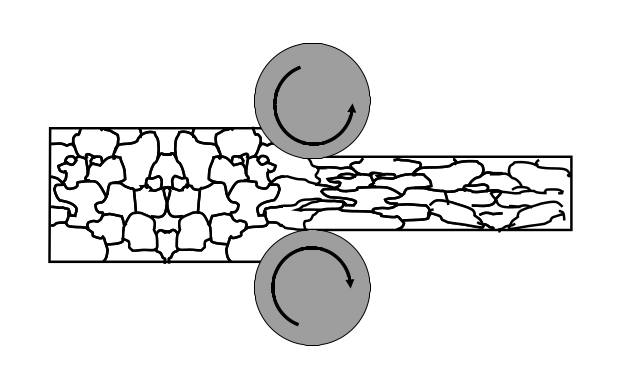
\includegraphics[scale=0.5]{rolling}

  \caption{Rolling (note the thinner grains)}
\end{figure}
\end{center}

\subsection{Work Hardening} 
As seen previously, work hardening occurs when a material is plastically deformed and released before it inevitably fractures.
Plastic deformation introduce many new dislocations.
Dislocations stop dislocations moving (and create new dislocations when moving).
The more dislocations there are, the harder it will be for them to move. 
This is, very scientifically, called a `traffic jam' and is what causes the strengthening due to work hardening.

\vspace{1cm}
Cold work is a name for the process of work hardening without heat i.e. rolling.
This causes a reduction in area as the material is because it is lengthening. 
Percentage cold work is hence the change in area over the original area. 

\begin{equation*}
  \frac{\Delta A}{A} \times 100
\end{equation*}

\subsection{Hardness}
Hardness is a resistance to a localised deformation. 
Hardness can be measured in many different ways, one popular one is the Rockwell Hardness Scales.
Geologists use Moh's which is basically "rate my rock 1-10" where 10 is diamond and 1 is Talc.

\begin{multicols}{2}
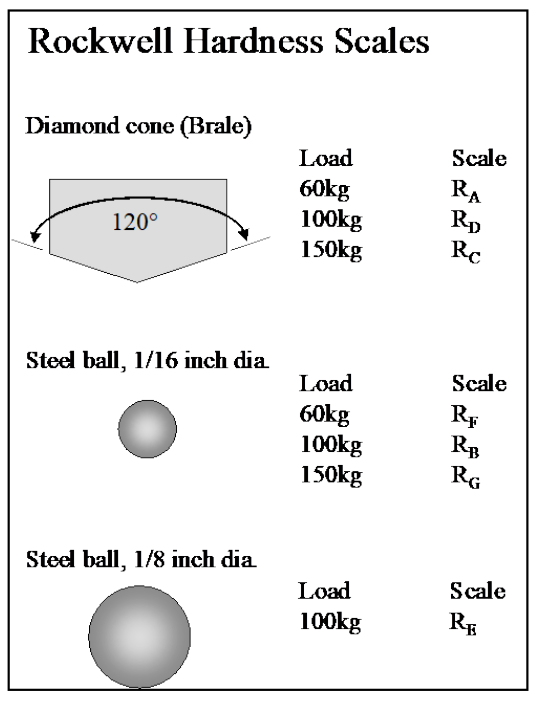
\includegraphics[scale=0.2]{rockwell}

The scales go from $R_a$ to $R_e$, where the different scales measure different levels of hardness.
Hardness has no units but you must state the scale you used i.e. 60$R_c$

You can test hardness with an indenter.
Where you make a plastic deformation with a known force behind it.

\end{multicols}

\subsection{Electrical Properties of Metals}
Electrical properties depend on atomic and crystal structures just as much as mechanical ones.
Resistivity depends on resistance (R), area (A) and length (L).
Resistance changes with temperature and so there is a second equation that has $\rho_0$ (the resistivity at room temperature), $\alpha$ (thermal co-efficient, given for each material) and $T$ (temperature).

\begin{equation*}
  \rho = \frac{RA}{L}
\end{equation*}

\begin{equation*}
  \rho_{\text{temp}} = \rho_0 (1+\alpha T)
\end{equation*}

Remember that resistivity will increase with cold work.
This is because conduction in metals is due to electron drift and the velocity of that drift.
Because work hardening causes increased dislocation density, electron movement is impeded.

Conductivity can be expressed as the product of $n$ (the number of electrons), $\abs{e}$ (the size of the charge on an electron and $\mu$ which is the `mobility of electrons'. 
\begin{equation*}
  \sigma = n \times \abs{e} \times \mu 
\end{equation*}

\subsection{Annealing}Annealing is a heat treatment that allows you to recover the ductility of a material (while sacrificing yield strength).
Annealing has three stages: Recovery, Recrystallisation and Grain Growth.
We will discuss each.

\begin{figure}[h]
  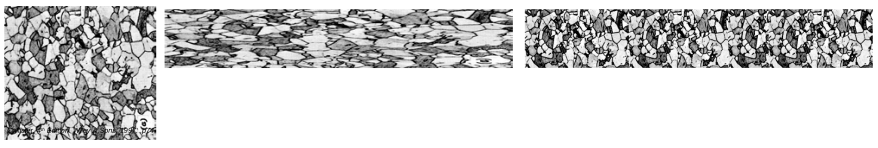
\includegraphics[scale=0.4]{annealing}
  \caption{From left to right: untreated, rolled, rolled and annealed}
\end{figure}

\subsubsection{Recovery}
In this stage, the material recovers from the work-hardening. 
The dislocation density does not change but rearranges to a lower energy configuration.

\subsubsection{Recrystallisation}
In the second stage, the metal is strain free.
New `baby grains' nucleate at the grain boundaries.
The driving force is the stored strain in the dislocations.
These new grains expand until they are equiaxed with low dislocation density.
Total recrystallisation occurs when just fully equiaxed.

\subsubsection{Grain Growth}
You can leave them to continue to grow for maximum ductility but this step is optional. 
You can choose to make the metal more ductile with larger grains or leave it to be stronger.

\subsection{Recrystallisation Temperature}
The rate of recrystallisation is proportional to temperature. 
There exists a `recrystallisation temperature' at which: a 50\% cold worked metal will just fully recrystallise in one hour.
Cold work less than 50\% will take longer. CW=50\% but lower temp will take longer.
Some examples are:

\begin{tabular}{c|c|c}
  Metal & Melting temperature $(^\circ C)$ & Recrystallisation temperature $(^\circ C)$ \\
  \hline
  Lead & 327 & -4 \\
  Aluminium & 660 & 80 \\
  Copper & 1085 & 120 \\
  Iron & 1538 & 370 \\
\end{tabular}

\subsubsection{Hot Work}
Hot work (i.e. forging) is work done to a metal above the recrystallisation temperature.
At this point, plastic deformation and recrystallisation happen at the same time. 
This means it won't be work hardened or it will be but it will be done at the same time.

\subsubsection{Diffusivity}
Diffusion is the movement of atoms through the lattice.
Lattice atoms (or substitutes) move via vacancy diffusion.
Interstitials `jump' positions by interstitial diffusion.

Diffusivity is a measure of how easily atoms can move.
Diffusivity (D) behaves according the Arrhenius equation (just like recrystallisation).
\begin{equation*}
  D = D_0 e^{\frac{-Q}{RT}}
\end{equation*}

\section{Phase diagrams and Alloying}
\subsection{Phases}
A phase is a component within a system that has uniform physical characteristics. 
In high school (and before) you were introduced to the typical Gas, Liquid and Solid (and maybe Plasma and Bose-Einstein Condensate).

\subsection{Solid Solutions}
There are two types of solid solution (in this course). 
Interstitial Solid Solutions and Substitutional solid solutions.
These two types have a number of different properties:

Interstitial Solid Solutions 
\begin{enumerate}
  \item Solute atom must be small (relative to solvent atom)
  \item Always have a solubility limit (limited interstitial spots)
\end{enumerate}

Substitutional Solid Solutions
\begin{enumerate}
  \item Similar Atomic Radius 
  \item Similar Crystal Structure (HCP, FCC etc.) 
  \item No Solid Solubility limit for some metals
\end{enumerate}

\subsection{Binary Isomorphous Phase Diagram}
This is a two metal (binary) single shape (i.e. FCC, isomorphous) phase diagram.
Here you can see the graph of temperature against weight percent Ni for a Cu solution.
Clearly, when $\alpha$ is 100\% copper it melts at the melting point of copper, 1085$^\circ C$ but when $\alpha$ is 100\% nickel, it melts at the melting point of nickel 1453$^\circ C$.
For any other composition, $\alpha$ will melt at a range of temperatures.
This is what we are graphing in a phase diagram.

\begin{center}
  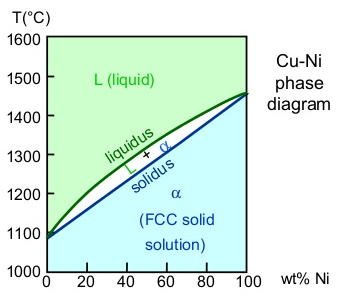
\includegraphics[scale=0.5]{binaryisomorphous}
\end{center}

\subsection{The Lever Rule}
The lever rule lets you calculate percentage makeups of the alloys and their phases.
To calculate the percentage of each phase at a given temperature:
\begin{enumerate}
  \item Place Pivot (always at the overall alloy composition)
  \item Draw the tie-line
  \item Draw on the phase symbols 
  \item Calculate Lengths
\end{enumerate}

\subsubsection{What are the compositions of each phase?}
Phases are oppposite, composition is on the `right' side.

To calculate the amount of each alloy in each phase, look at where the tie-line intersects with the solidus, that will be the percentage amount of Ni (or whatever is on the x axis).
You can then calculate the amount of the other metal by subtracting from 100. 

The intersection with the liquidus will give you the percentage of Ni in the liquid state and so on.
This is a useful tool for all phase diagrams but is especially easy to use in this case.


\subsection{Binary Eutectic Phase Diagram}
\begin{center}
  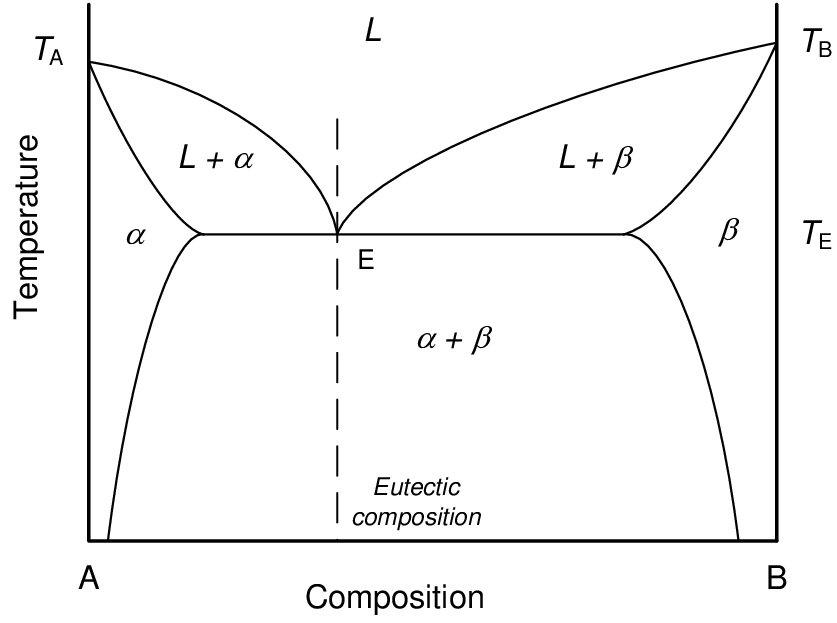
\includegraphics[scale=0.5]{binaryeutectic}
\end{center}

\subsubsection{The Eutectic Point}
The Eutectic Point is a point at which the alloy has its own freezing or melting point.
This is clearly seen on the graph where the two lines meet with the $\alpha$ and $\beta$ section.
The Eutectic reaction is when a liquid phase transforms into two solid phases ($\alpha+\beta$)

\begin{equation*}
  L_{EUT} \underset{\text{heat}}{\stackrel{\text{cool}}{\rightleftharpoons}} \alpha + \beta 
\end{equation*}

\subsubsection{Microstructure Development}
The microstructure of metals formed will vary greatly but noticably will form equiaxed grains of one element with grains of the other at the boundaries or layers of each metal.
Metals that form large grains on grain boundaries are called proeutectic.

\section{Strengthening mechanisms}
In 121, when we say strength we are generally referring to yield strength.
This is the stress at which a material will begin to plastically deform.  

\begin{equation*}
  \text{strength} \approx \sigma_y
\end{equation*}

\subsection{Work Hardening}
Any plastic deformation increases strength.
This is because for plastic deformation to occur, dislocations have to move. 
Plastic defomation increases dislocation density which causes a `dislocation traffic jam' and the yield strength will increase.

\subsection{Grain Size Reduction}
Reducing the grain size will increase the yield stress of a material (by the Hall-Petch equation).
We can do this by controlling the amount of cold work before recrystallisation, and then controlling the aount of grain growth after recrystallistion (see annealing).

\subsection{Solid Solution Strengthening}
Solid Solution Strengthening involves making an alloy with a bigger or smaller atom to distort the slip planes of the parent lattice.
Distorting the parent lattice means it will be harder for dislocations to move so yield strength will increase.
Hence, the maximum yield stress (and resistivity) will occur at the optimal combination of metals.
(Remember, ductility is (sort of) the opposite of strength so the graphs will be opposite here)

\subsection{Multiphase Strengthening}
Any boundary can stop dislocation movement: a grain boundary or \textit{a boundary between two phases}. 
Multiphase strengthening is choosing an alloy to maximise the number of boundaries.
You can choose an alloy to maximise the number of boundaries most easily by increasing the amount of eutectic. 
This is because the layers of a eutectic solid are exactly what we are looking for.

A eutectic solid (a metal with the eutectic metal combination) cooled to solid will have the following properties:
very high yield strength, lower ductility (In the CuAl example, still ductile). Pearlite like layers.

\subsection{Strengthening Methods for Steel}
\subsubsection{Martensite}
By quenching from the Austenite region we can form a phase called Martensite.
No diffusion is required (because it is a displacive or shear transformation) so this transformation is almost instant.

\begin{itemize}
  \item BCT $\implies$ No slip systems $\implies$ Hard and Brittle
  \item It is a super-saturated solid solution of C in Fe
  \item It is METASTABLE
\end{itemize}

\begin{marginfigure}
  \vspace{-1cm}
  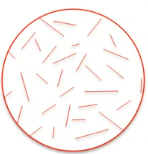
\includegraphics[scale=0.3]{martensitestructure}
\end{marginfigure}

\begin{marginfigure}
  \vspace{-2cm}
  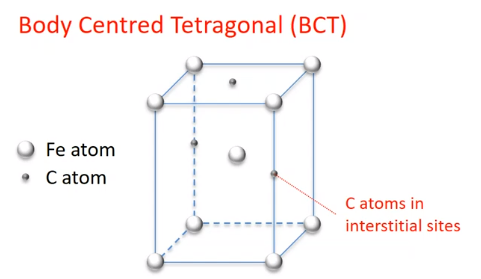
\includegraphics[scale=0.3]{martensitecell}
\end{marginfigure}

\subsubsection{Tempered Martensite}
When you temper martensite, you get a very fine dispersion of Fe$_3$C particles in a ductile ferrite matrix.
Tempered Martensite contains NO actual martensite.
It has been heat treated (tempered) to `push' the metastable phase into stable phases.
Note that Fe$_3$C$+\alpha$ is \textbf{not} pearlite. 
Recall that we only get pearlite when cooling from the austenite region.
This is hence a new compound that we call Tempered Martensite.
Below 723$^\circ$C, this reaction will happen:
\begin{equation*}
  M \rightarrow \alpha + \text{Fe}_3\text{C}
\end{equation*}
In this reaction, C diffuses out of the BCT structure of Martensite into Fe$_3$C, and the BCT structure relaxes into BCC Iron ($\alpha$).
Below is the resulting microstructure/s:

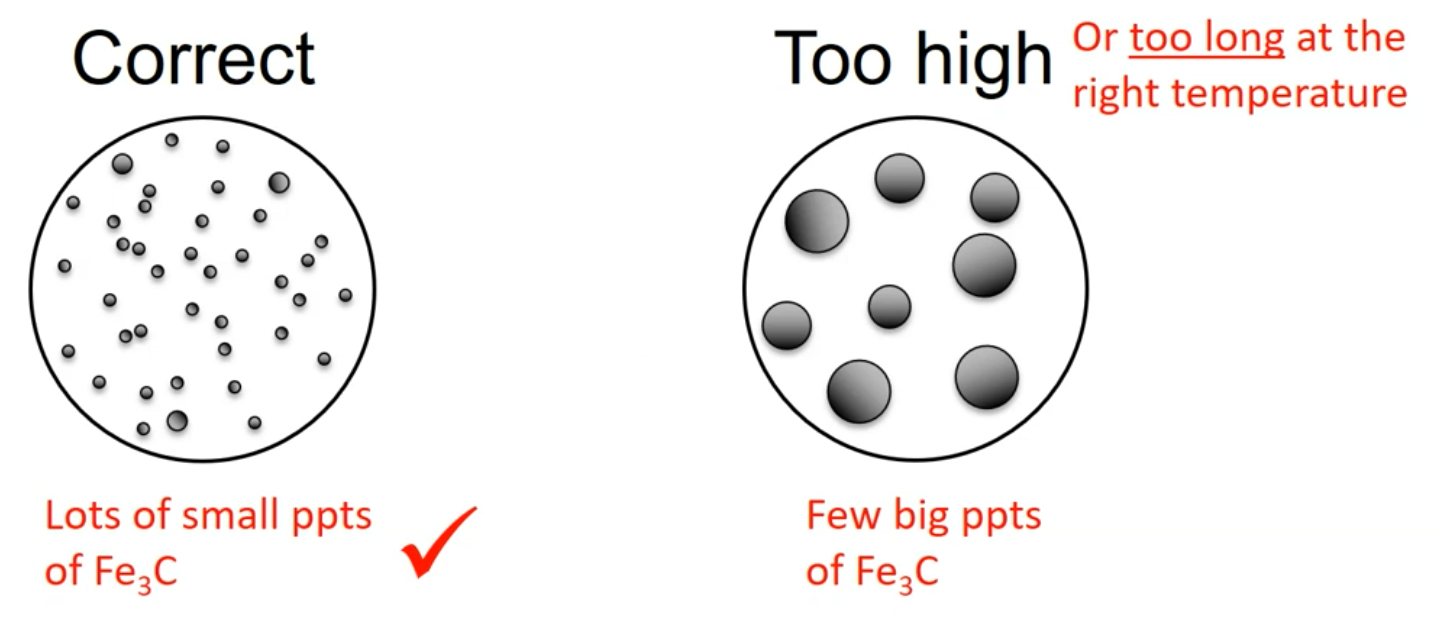
\includegraphics[scale=0.3]{martensite}

Tempered Martensite Properties:
\begin{itemize}
  \item Optimum Strength for a steel with sufficient ductility to still be tough
\end{itemize}

\subsubsection{Spheroidising of Steels}
The spheroidisation of Steel is a heat treatment that makes it more ductile.
It only works for steels that contain pearlite i.e. have been slowcooled and have a hight amount of Carbon (0.5-1 \%).

\begin{center}
Heating to $700^\circ C$ and holding for several hours transforms the layers of $Fe_3C$ into spheres.
\end{center}


\subsection{Time-Temperature-Transformation (TTT) Curves }
A TTT curve tells us how fast is fast cooling. 
Generally, we do this to figure out what phases will form in a metal cooled from one temperature to another in a given time. 
It graphs temperature against time (generally log time)
It is useful but limited, it cannot tell you what happens in the bottom right (dotted point).  

The `curvy' curve is the start and finish lines of the pearlite transformation from austenite (oft included is a `50\%' complete line, which will be 50\% Austenite and 50\% Pearlite).
Pearlite exists on a spectrum between 'coarse' and 'fine', above 'the nose' (farthest left point of the start line) will form coarse Pearlite and below that will form fine Pearlite. 
Below that, the microstructure formed will be Bainite (not important for 121).
Below that is the Martensite Start Line, this will be where Martensite is formed.

It's important to remember that these only really make sense with "Isothermal heat treatment". 
This means the line travels straight horizontally. 
This is an assumption that is rarely true in real life.

\begin{theorem*}
In 121, we only discuss a steel with a eutectoid composition (0.8\% C).
\end{theorem*}

For a steel of eutectoid composition (0.8\% C),
\begin{center}
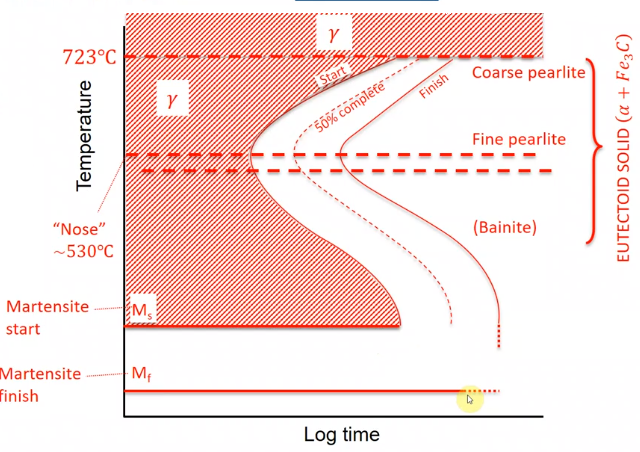
\includegraphics[scale=0.5]{ttt}
\end{center}

\subsubsection{Steel Summary}
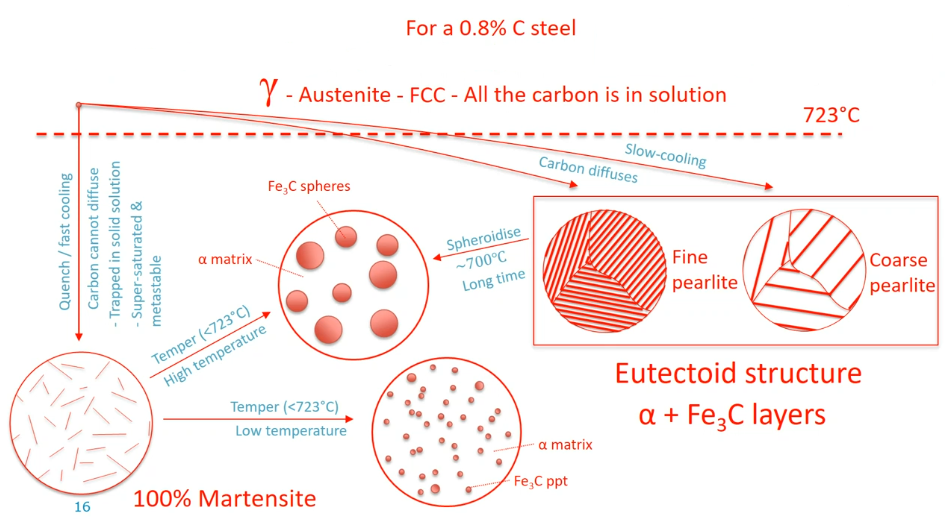
\includegraphics[scale=0.4]{steelsummary}

A steel is an alloy of Fe and C.
Steels are widely used in engineering because they are cheap and effective. 
Steels are interstitial solids meaning each phase has a fixed solubility of Carbon.

\begin{theorem*}
  \textbf{Ferrite} ($\alpha$)

  Ferrite has a BCC structure and exists on the far left of the phase diagram (maximum solubility of 0.02\%).
  Ferrite is ductile, magnetic (ferrous) and exists between room temperature and 910$^\circ C$.
\end{theorem*}

\begin{theorem*}
  \textbf{Austenite} ($\gamma$)

  Austenite has an FCC structure and a maximum solubility of 1.7\%.
  It is also ductile but non-magnetic.
\end{theorem*}

\begin{theorem*}
  \textbf{Cementite} ($Fe_3C$)

  Cementite is not a phase but a compound of fixed composition.
  It is very brittle and hard.
\end{theorem*}

\begin{theorem*}
  \textbf{Pearlite} ($P$)

  Pearlite is the microconstituent of Steel that forms at the eutectoid composition (0.8\%).
  It consists of layers of ductile ferrite ($\alpha$) and brittle cementite ($Fe_3C$).
\end{theorem*}

\begin{theorem*}
  \textbf{Martensite} ($G$)

  Martensite is a super-saturated solid solution of C in Fe that is BCT and hence hard and brittle.
  It is metastable and formed from quenching. 
\end{theorem*}

\section{Engineering ceramics and glasses}
Ceramics are usually combinations of metals and non-metals (sometimes there can be metalloids in there). 
The bonding is either ionic or covalent (or somewhere inbetween).
They have their own structures (similar to that of metals) and their own processes. 
Ceramics are generally very strong in compression but weak in tension but their main fault is that they are extremely brittle.

\subsection{Ceramic Structures}
\subsubsection{Covalent Bonds}
In a covalent bond, electrons are shared between atoms. 

\textbf{Properties}
\begin{itemize}
  \item Very strong
  \item Very directional
  \item Fixed bond angle 
\end{itemize}

\subsubsection{Ionic Bonds}
In an ionic bond, valence electrons are donated from the positive cation to negatively charged anion.

\textbf{Properties}
\begin{itemize}
  \item Very strong 
  \item Non-directional
\end{itemize}

With these bonds, there are some general structures that can be formed.
Remember,
\begin{itemize}
  \item Anions do not touch other anions
  \item Cations and anions are touching
  \item Charges are balanced
\end{itemize}

\subsubsection{Sodium Chloride Structure}
\begin{center}
  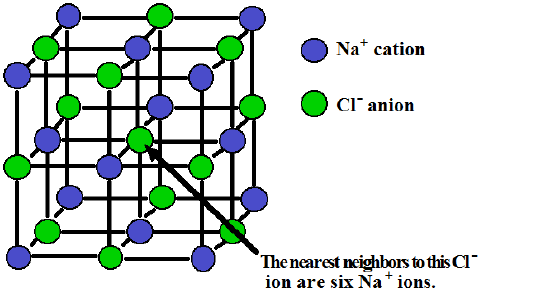
\includegraphics[scale=0.5]{naclstructure}
\end{center}

NaCl has this structure (hence the name).
It is two interlocking FCC structures. 
Ceramics with this structure are commonly used in refactories (melting steel in a steel bucket).

\textbf{Properties}
\begin{itemize}
  \item General formula $AB$
  \item Co-ordination number for each type of ion = 6
  \item Has Cation on every edge and in the center
  \item Has Anion on every face and corner 
  \item $a = 2(R_C + R_A)$
\end{itemize}

\subsubsection{Perovskite Structure}
\begin{center}
  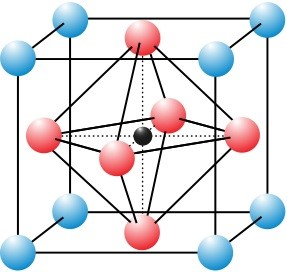
\includegraphics[scale=0.4]{perovskitestructure} \end{center}
It gets more complicated when the charges are uneven and there is one type of cation.
\begin{itemize}
  \item $ABO_3$
  \item 'bottom' is slightly negative because smaller cation is shifted up, so structure has a permanent dipole 
  \item Has larger cation (in size) at every corner
  \item Has smaller cation in the middle 
  \item Has anion on every face
\end{itemize}

\subsection{Silicate Structures}
Rocks, soils, clays and sand are all silicate structures.
They are based on joining up the $SiO_4^{4-}$ tetrahedra.
If only some of the oxygens in silicate are joined to another tetrahedron you get chains, rings or sheets.
If they are all bonded, then you get 3D structures such as Quartz.

You can draw these using triangles with a dot. 

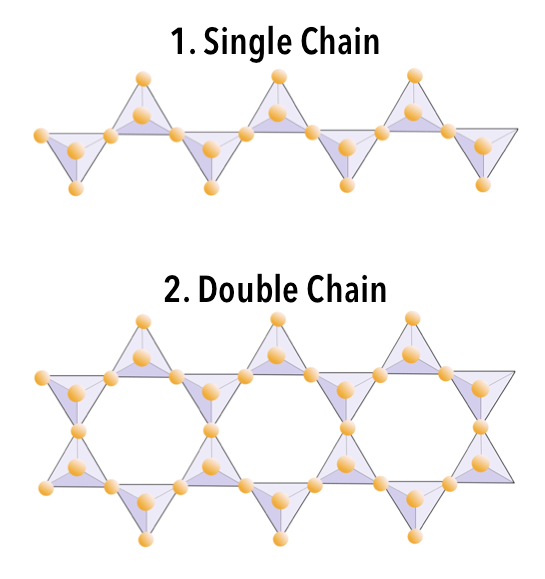
\includegraphics[scale=0.2]{silicatestructure}

\subsection{Fracture toughness of ceramics}
Plastic deformation (slip/dislocation movement) in ceramics is practically impossible because of the nature of ionic bonds.
Ionic bonds cannot break and reform (negative against negative) which leads to immediate fracture. 

Additionally, the gradient of a stress-strain curve for a ceramic materials is very high.
Remember that this is all about how much you can stretch the inter-atomic bonds of a material and the bonds in ceramics are very strong.
Ceramics are almost completely brittle.

The theoretical strength of a ceramic is very high but is never even close.
This is because (once again) of \textbf{imperfections}. 
Where in metals we have dislocations, in ceramics we have pores, cracks and scratches.

Porosity is very important for a ceramic.
Porosity reduces strength because it; 1, reduces cross-sectional area and 2, pores act as stress concentrators. 

In summary:
\begin{itemize}
  \item No plastic deformation / completely brittle
  \item Low toughness ($\approx$ 1/50 metals, Even a small pore has a LARGE effect)
  \item Highly likely that ceramics contain weakening porosity. 
  \item Very strong in compression
\end{itemize}

\subsubsection{Toughening Mechanisms}
So how can we fix these issues?

\begin{itemize}
  \item Reduce porosity (densifying)
  \item Reinforce with something else (i.e. steel rebar)
  \item Transformation Toughening
\end{itemize}

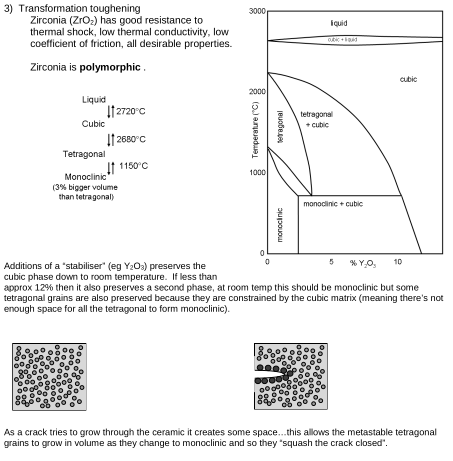
\includegraphics[scale=0.6]{transformationtoughening}

\subsection{Processing Ceramics}
Unlike metals, we cannot melt and cast ceramics (what would we melt them in??).
They are not plastic so they cannot be shaped. 
How do we process them?

\begin{itemize}
  \item Hydroplastic Forming
  \item Slip casting 
  \item Powder Pressing
  \item Sintering
\end{itemize}

Hydroplastic forming is simply adding water to the material and shaping it. 
With a little water, clay becomes very plastic.

Slip casting comes when you add even more water and you get a slurry or \textit{slip} that can be poured into a cast.

After it is formed, ceramics need drying and firing in a kiln.
This is a complex process, one of the things that happens is vitrification.
During vitrification, some of the components melt and flow around ceramic particles and solidify as glass. 

\textbf{Advanced Ceramics}

Powder pressing involves the pressing (uniaxial, double-action or isostatic (isostatic is all directions)) of a powder (green compact) into a ceramic (this is densifying).
Sintering is a heat treatment process that makes the material denser.
After heating, the material shrinks and this reduces porosity.
The driving force for sintering is reducing the surface area.
Sintering is modeled by the arrheneus equation so:
\begin{equation*}
  \frac{d\rho}{dt} = \frac{1}{G^n} \times Ae^{(\frac{-Q_s}{RT})}
\end{equation*}

\subsection{Glass}
Glasses are ceramics with no long range order commonly based on silica. 
Glass is non-crystalline (does not have a crystal structure) and hence amorphous.

Glass can be formed in many ways.
Glass forming oxides can form networks with no long range order.
Network modifiers disrupt networks to give particular properties (e.g. lower viscosity).

Properties:
\begin{itemize}
  \item Excellent optical properties
  \item High chemical stability 
  \item Electrical insulator (no free electrons)
  \item Thermal properties (expansion) can be altered by composition
  \item Extremely brittle (ceramic)
\end{itemize}

\subsection{Glass Processes} 
\subsubsection{Tempering}
Tempering can improve fracture toughness.
THe surface region is put into compression by thermal or chemical techniques and there is a residual tension in the middle of the glass.
This means that the glass will break into small pieces (which is much safer than giant shards).

The general steps are:
\begin{itemize}
  \item Heat glass above $T_g$
  \item Spray glass with water (causes shrinkage on the outside)
  \item Outer layer ccools faster
  \item Inner material cools slower (pulls the outer layer into compression)
\end{itemize}

\subsubsection{Annealing}

\section{Polymers}
Materials with structures made up of repeating molecular units are called polymers.
In 121, we will only consider those polymers made up of Carbon (organic).
The repeating units of a polymer are called `mers'. 
These repeating units are the covalently bonded together to form \textbf{long} chains.

\subsection{Polymerisation}
\begin{itemize}
  \item The double bond between C atoms "opens up"
  \item A single covalent bond forms in its place 
  \item Each C atom can then bond to another molecule/atom
  \item This repeats many times to form a chain
\end{itemize}

The degree of polymerisation (DP) is a measure of how much it has polymerised i.e. \textbf{how long the chain is}.
It can be calculated by dividing the average molecular weight of chains in the polymer by the molecular weight of the mer.
The polymerisation reaction produces chains of variable length so the molecular weight is always expressed as an average value.
A higher DP means a longer chain.

\subsubsection{How DP affects strength}
Between the separate polymer chains in a polymer compound there are much weaker secondary bonds (Van der Waal's forces). 
These still contribute to the mechanical properties along with the tangling between chains.
Short chains are easy to break because they themselves break easily and chains can slide past each other under load.
Longer chains have lots of secondary bonds (Van der Waal's forces) and make it more difficult to get chains to slide past one another (due to chain tangling).

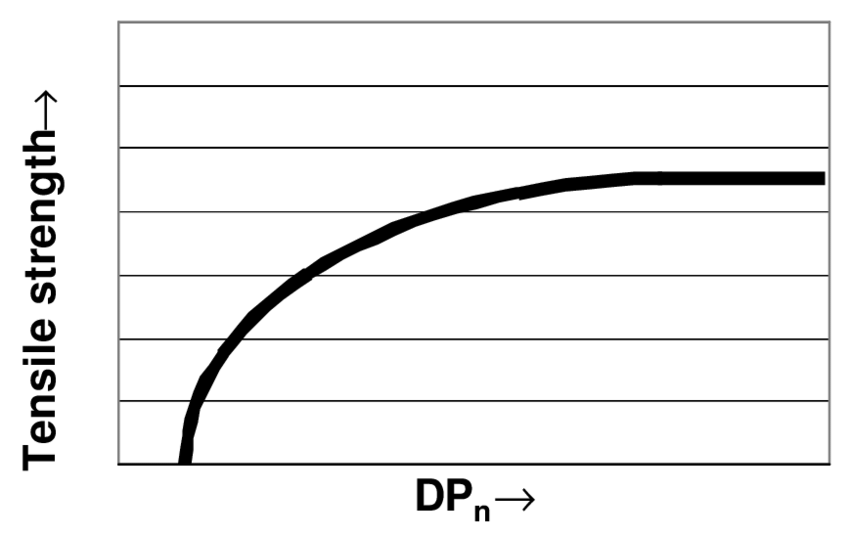
\includegraphics[scale=0.3]{strengthagainstdp}

The graph reaches a maximum because at that point you start breaking the actual molecule itself (polymer bonds).
The graph starts above zero because chains are two short for secondary bonding so they have no solid boundaries.

\subsection{Polymer Description}
The things that can be used to describe a polymer are: 
\begin{itemize}
  \item Its mer/s
  \item Chain Structure (how the mer/s is/are patterned) 
  \item How it connects to other polymers
  \item Thermoplastic/Thermosetting/Elastomer etc.
  \item Amorphous vs Crystalline 
\end{itemize}

\subsubsection{Mer Traits}
A mer is the repeating unit (or units) in a polymer chain. 
They can be described by a number of things.
The most typical mers in 121 are made up of just hydrogen and carbon (hydrocarbons) but can also contain other things like halogens or other sidegroups.
Large sidegroups will have a large effect on the final polymer. 
Very large sidegroups can do things like make it transparent.

\subsubsection{Chain Structures}
\textbf{Homopolymers} have one mer that repeats along the chain.

\textbf{Co-polymers} have two or more different mers.


\begin{multicols}{2}
  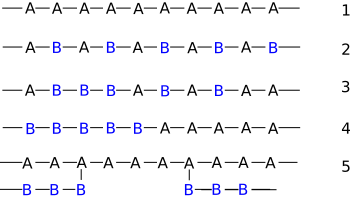
\includegraphics[scale=0.5]{copolymers}
\begin{enumerate}
  \item Homopolymer
  \item Alternating 
  \item Random 
  \item Block 
  \item Graft
\end{enumerate}
\end{multicols}

\subsubsection{Polymer Shape}
Polymers can be linear, branched or cross-linked.

\textbf{Linear}
polymers are simply repeating units end-to-end with no side-groups or anything.
These are flexible and have a higher density because they can pack closely together.

\textbf{Branched}
polymers have a main polymer, to which side branches are connected.
This reduces how close the chains can get thus reducing density.

\textbf{Cross-linked polymers}
are linear polymer chains that are joined by covalently bonded `chain segments'.
Cross-links prevent relative movement between chains that means they are stiff, hard and strong. 

\subsubsection{Other Classifications}
\textbf{Thermoplastic}

Thermoplastics can be melted and reshaped (they can be thermally deformed plastically).
Most importantly, this means they can be recycled.
When melted, they act as a viscous liquid.

They are linear or branched polymers with weak secondary bonds.
Heat increases thermal vibration of polymer chains which reduces secondary bonding and allows relative movement of the chains.

\textbf{Thermosetting}

These are cross-linked polymers that have the strong covalently bonded cross links that prevent flow. 
These materials will be harder and stronger than thermoplastics but cannot be melted.
When heated, these materials will burn and char. 

\textbf{Elastomers} 

These are structures made up of polymer chains that are twisted, kinked and coiled.
This means when they are stretched they can uncoil/unkink and extend but the cross-links will prevent permanent deformation (movement of chains).
The polymers will spring back to their original position after they are released. 
They have been deformed elastically.

\subsubsection{Bulk Polymer Structures}
This is how many polymer chains fit together. 
Like how FCC atoms build a larger metal structure, polymers build a larger structure except they are not usually organised.
They are normally just dumped out like a cup of rubber bands. 
This is called \textbf{Bulk Amorphous Structure}.

However, sometimes polymers are structured for a little bit (in a section).
This is called \textbf{Partial Crystallinity}.
Regions of structure are called "crystallites" and have much higher strength due to the higher concentration of secondary bonds. 
Note that complete crystallinity is not possible.

\section{Failure of materials}
\section{Corrosion of metals}
\section{Engineering composites}
\end{document}
